\section{Istruzioni per l'uso}
\subsection{Requisiti di sistema}
Descrizione di tutti i requisiti necessari a funzionamento dell'applicazione Premi.

\subsection{Guida all'installazione???}
Serve? Boh...

\subsection{Primo accesso}
Al primo accesso il sistema richiede l'autenticazione dell'utente qualora fosse già registrato al sistema, altrimenti fornisce la possibilità di creare un nuovo account.
\begin{figure}[h]
\begin{center}
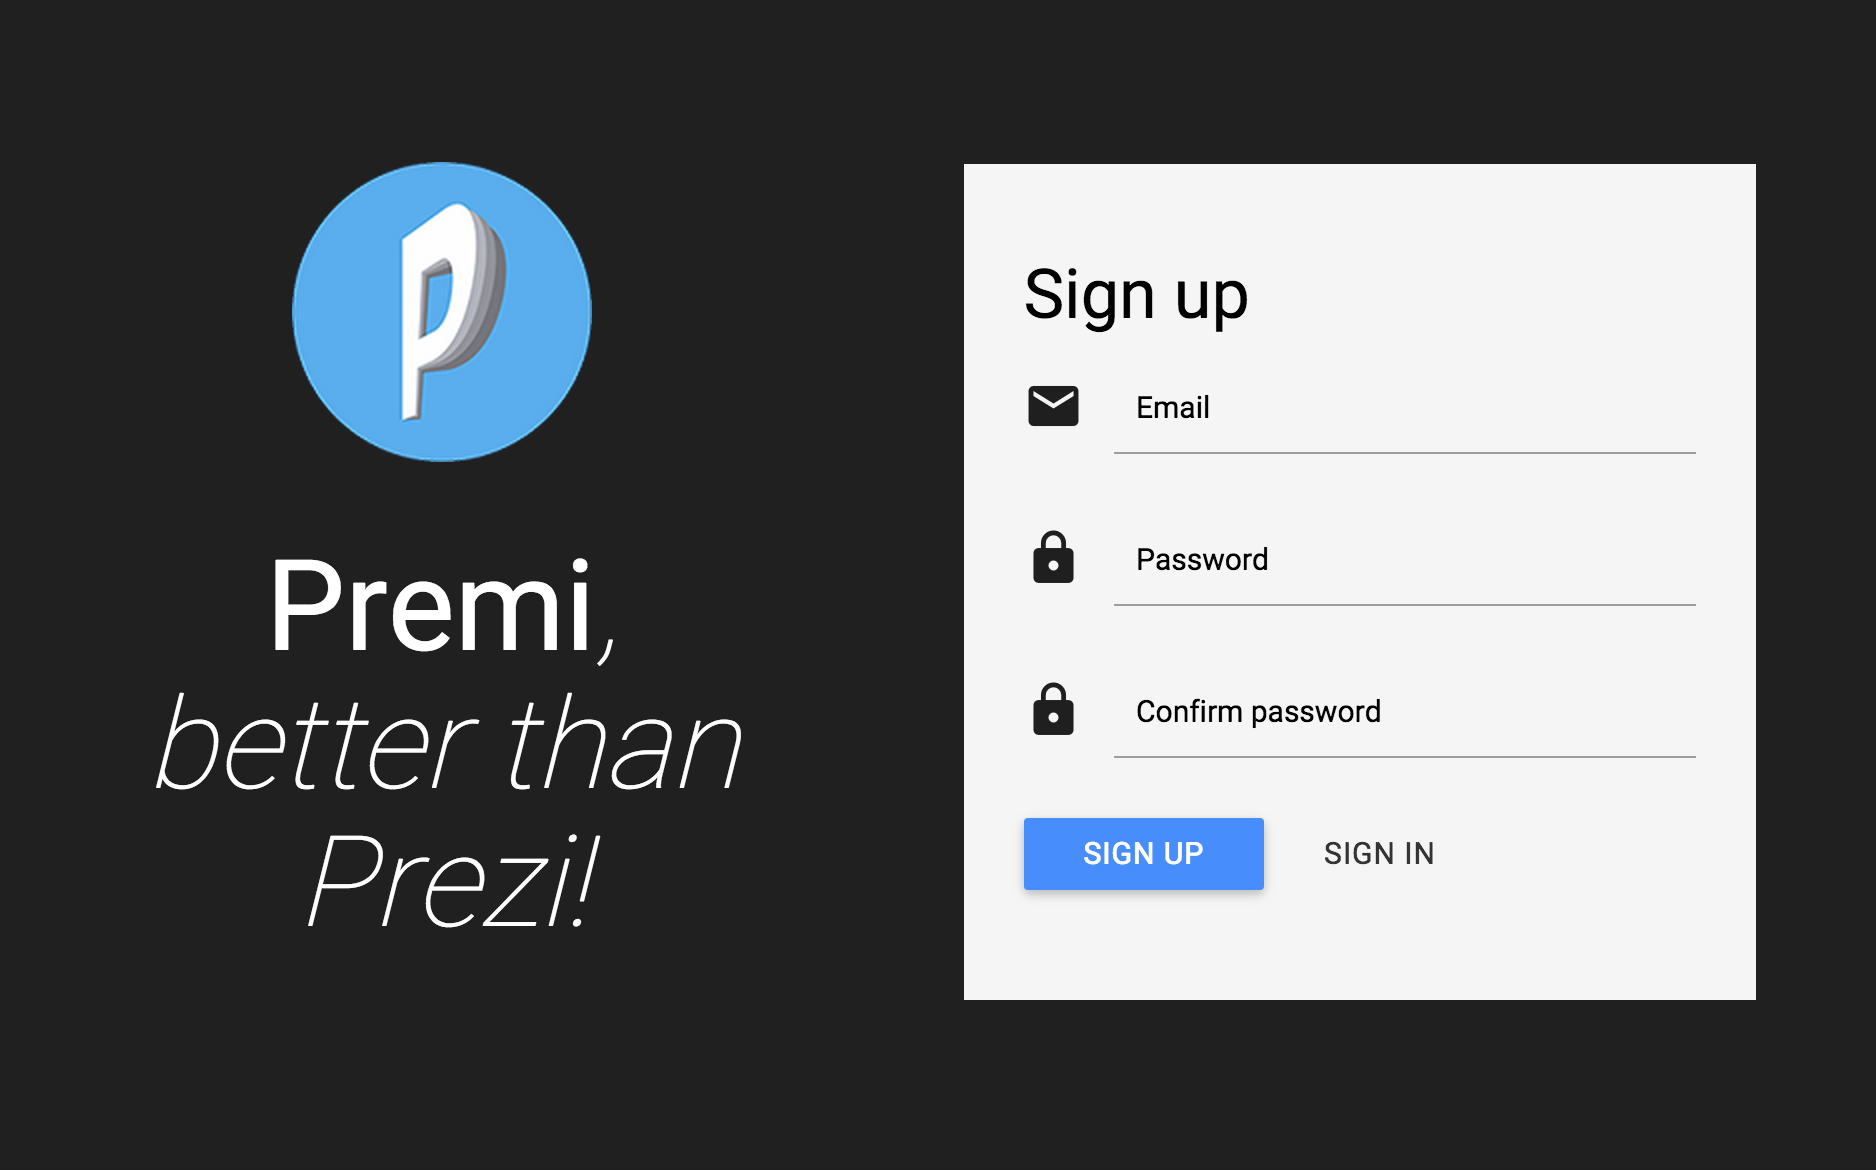
\includegraphics[scale=0.4]{img/signup.png}
\caption{Form di registrazione.}
\end{center}
\end{figure}

Per la creazione di un nuovo account i dati da inserire sono soggetti ad alcuni vincoli:
\begin{itemize}
\item Indirizzo email: deve essere un indirizzo valido;
\item Password: composta da almeno n. caratteri;
\item Conferma password: deve coincidere con il campo password precedente.
\end{itemize}
Per confermare la registrazione premere sul tasto "SIGN UP".
\begin{quote}
\textbf{Nota:} si potrebbero ricevere degli avvisi che notificano l'errato inserimento dei dati richiesti.
\end{quote}
Una volta completata la registrazione è necessario autenticarsi al sistema:
\begin{figure}[h]
\begin{center}
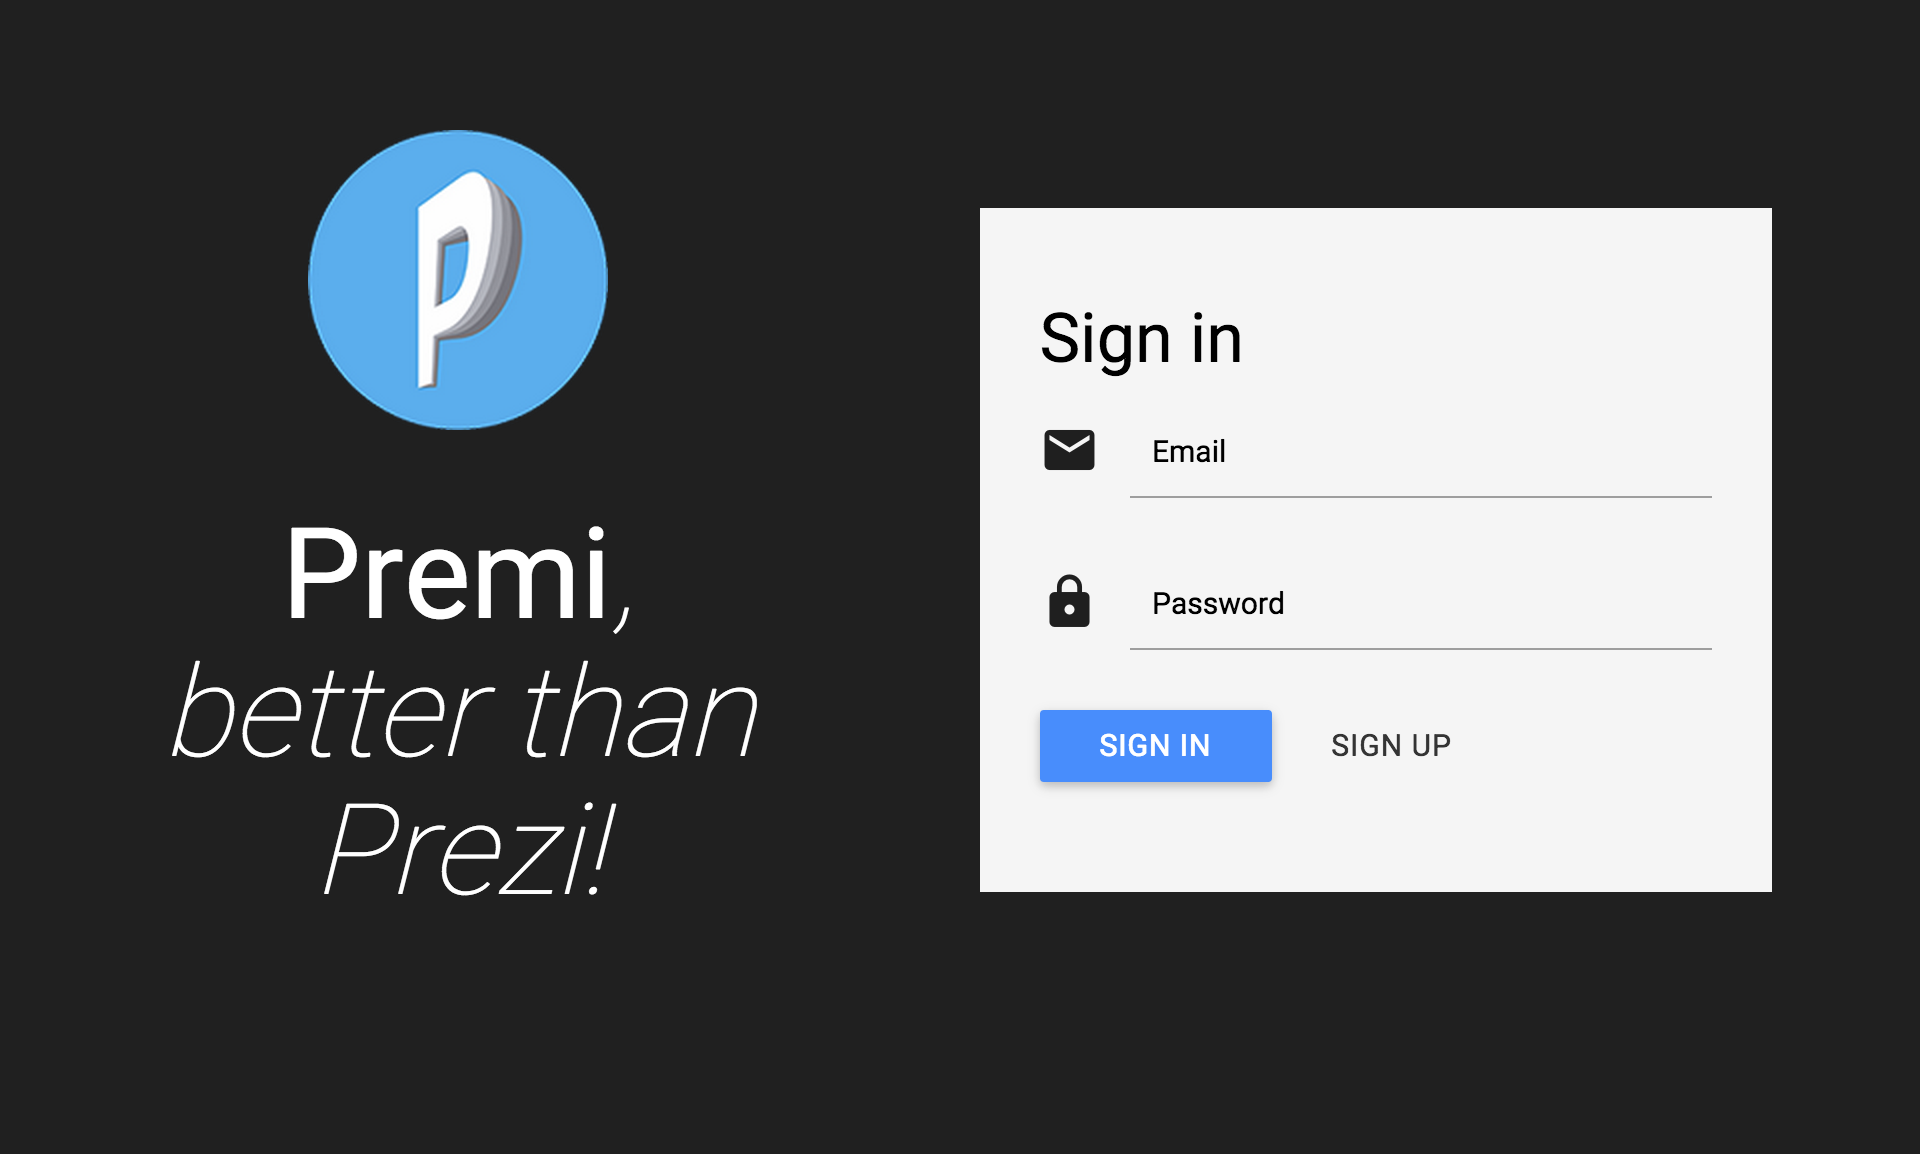
\includegraphics[scale=0.4]{img/signin.png}
\caption{Autenticazione al sistema.}
\end{center}
\end{figure}

\newpage
\subsection{Pannello di controllo dell'utente}
Una volta autenticati al sistema si accede al proprio pannello di controllo, all'interno del quale saranno visibili tutte le presentazioni finora create.
\begin{figure}[h]
\begin{center}
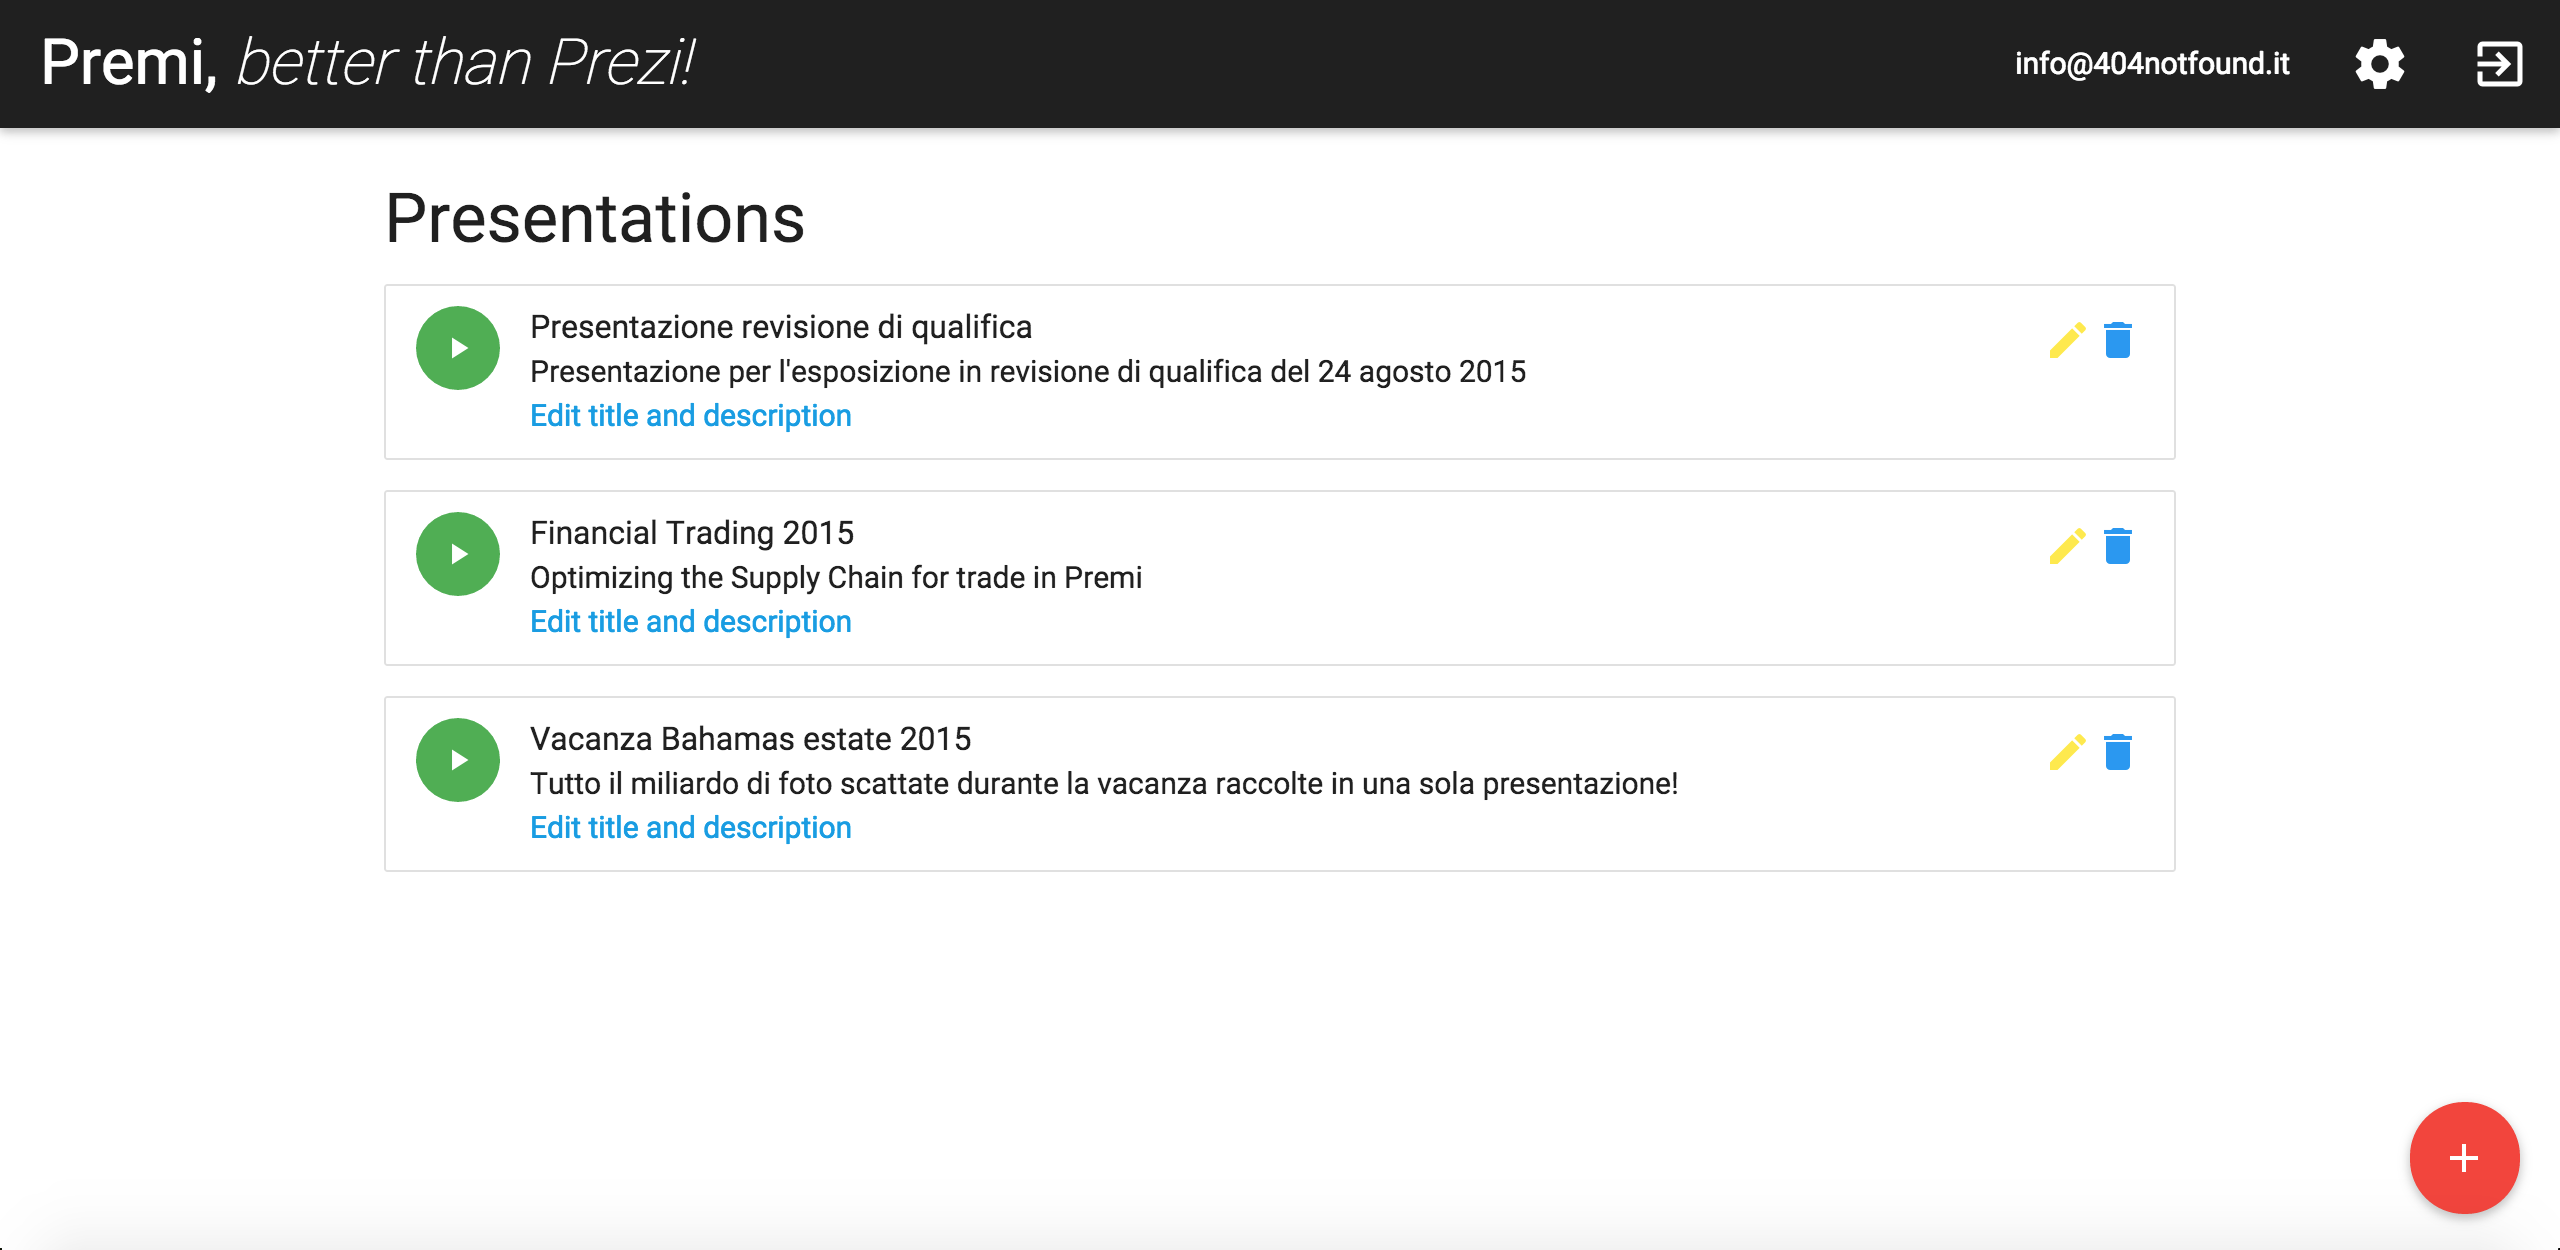
\includegraphics[scale=0.35]{img/dashboard.png}
\caption{Pannello di controllo utente.}
\end{center}
\end{figure}

Comandi:\\ \\
\begin{tabular}{ c l }
\parbox[c]{2em}{
\includegraphics[scale=0.6]{img/gear.png}} & Permette la modifica dei dati dell'account;\\
\parbox[c]{2em}{
\includegraphics[scale=0.6]{img/quit.png}} & Consente all'utente di disconnettersi dal sistema;\\
\parbox[c]{2em}{
\includegraphics[scale=0.4]{img/add.png}} & Permette la creazione di una nuova presentazione.\\
\end{tabular}

\newpage
\subsection{Creare una nuova presentazione}
\begin{figure}[h]
\begin{center}
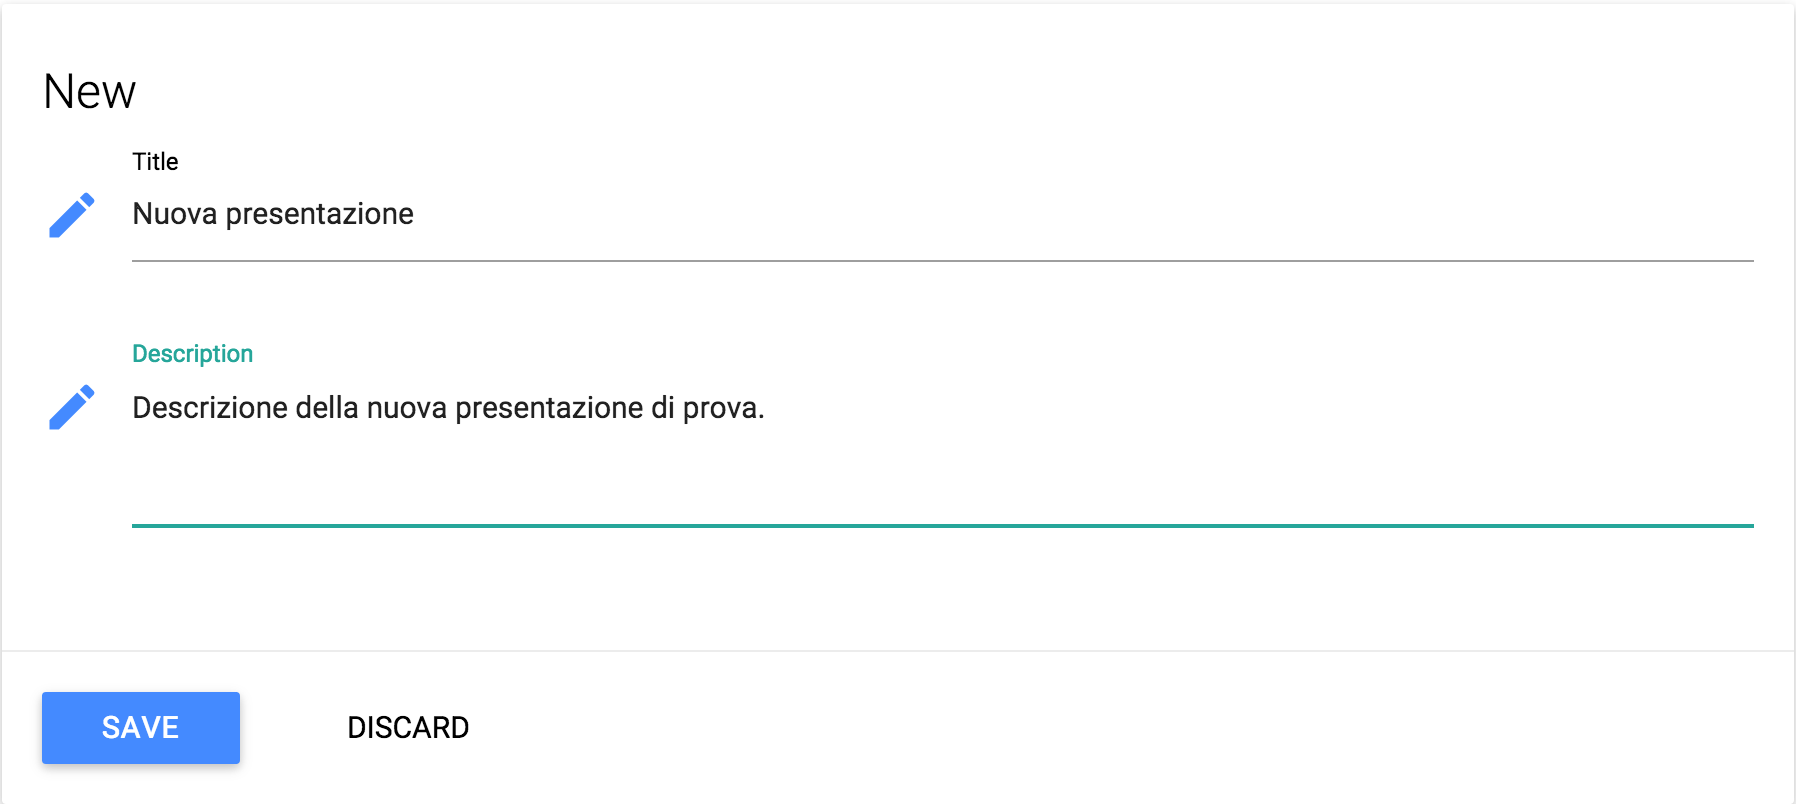
\includegraphics[scale=0.4]{img/new_pres.png}
\caption{Creazione nuova presentazione.}
\end{center}
\end{figure}

Per creare una nuova presentazione sarà sufficiente inserire il titolo e una descrizione, come visualizzato nella figura 4.
Una volta creata la presentazione questa verrà automaticamente aggiunta all'elenco delle presentazioni personali.
\begin{figure}[h]
\begin{center}
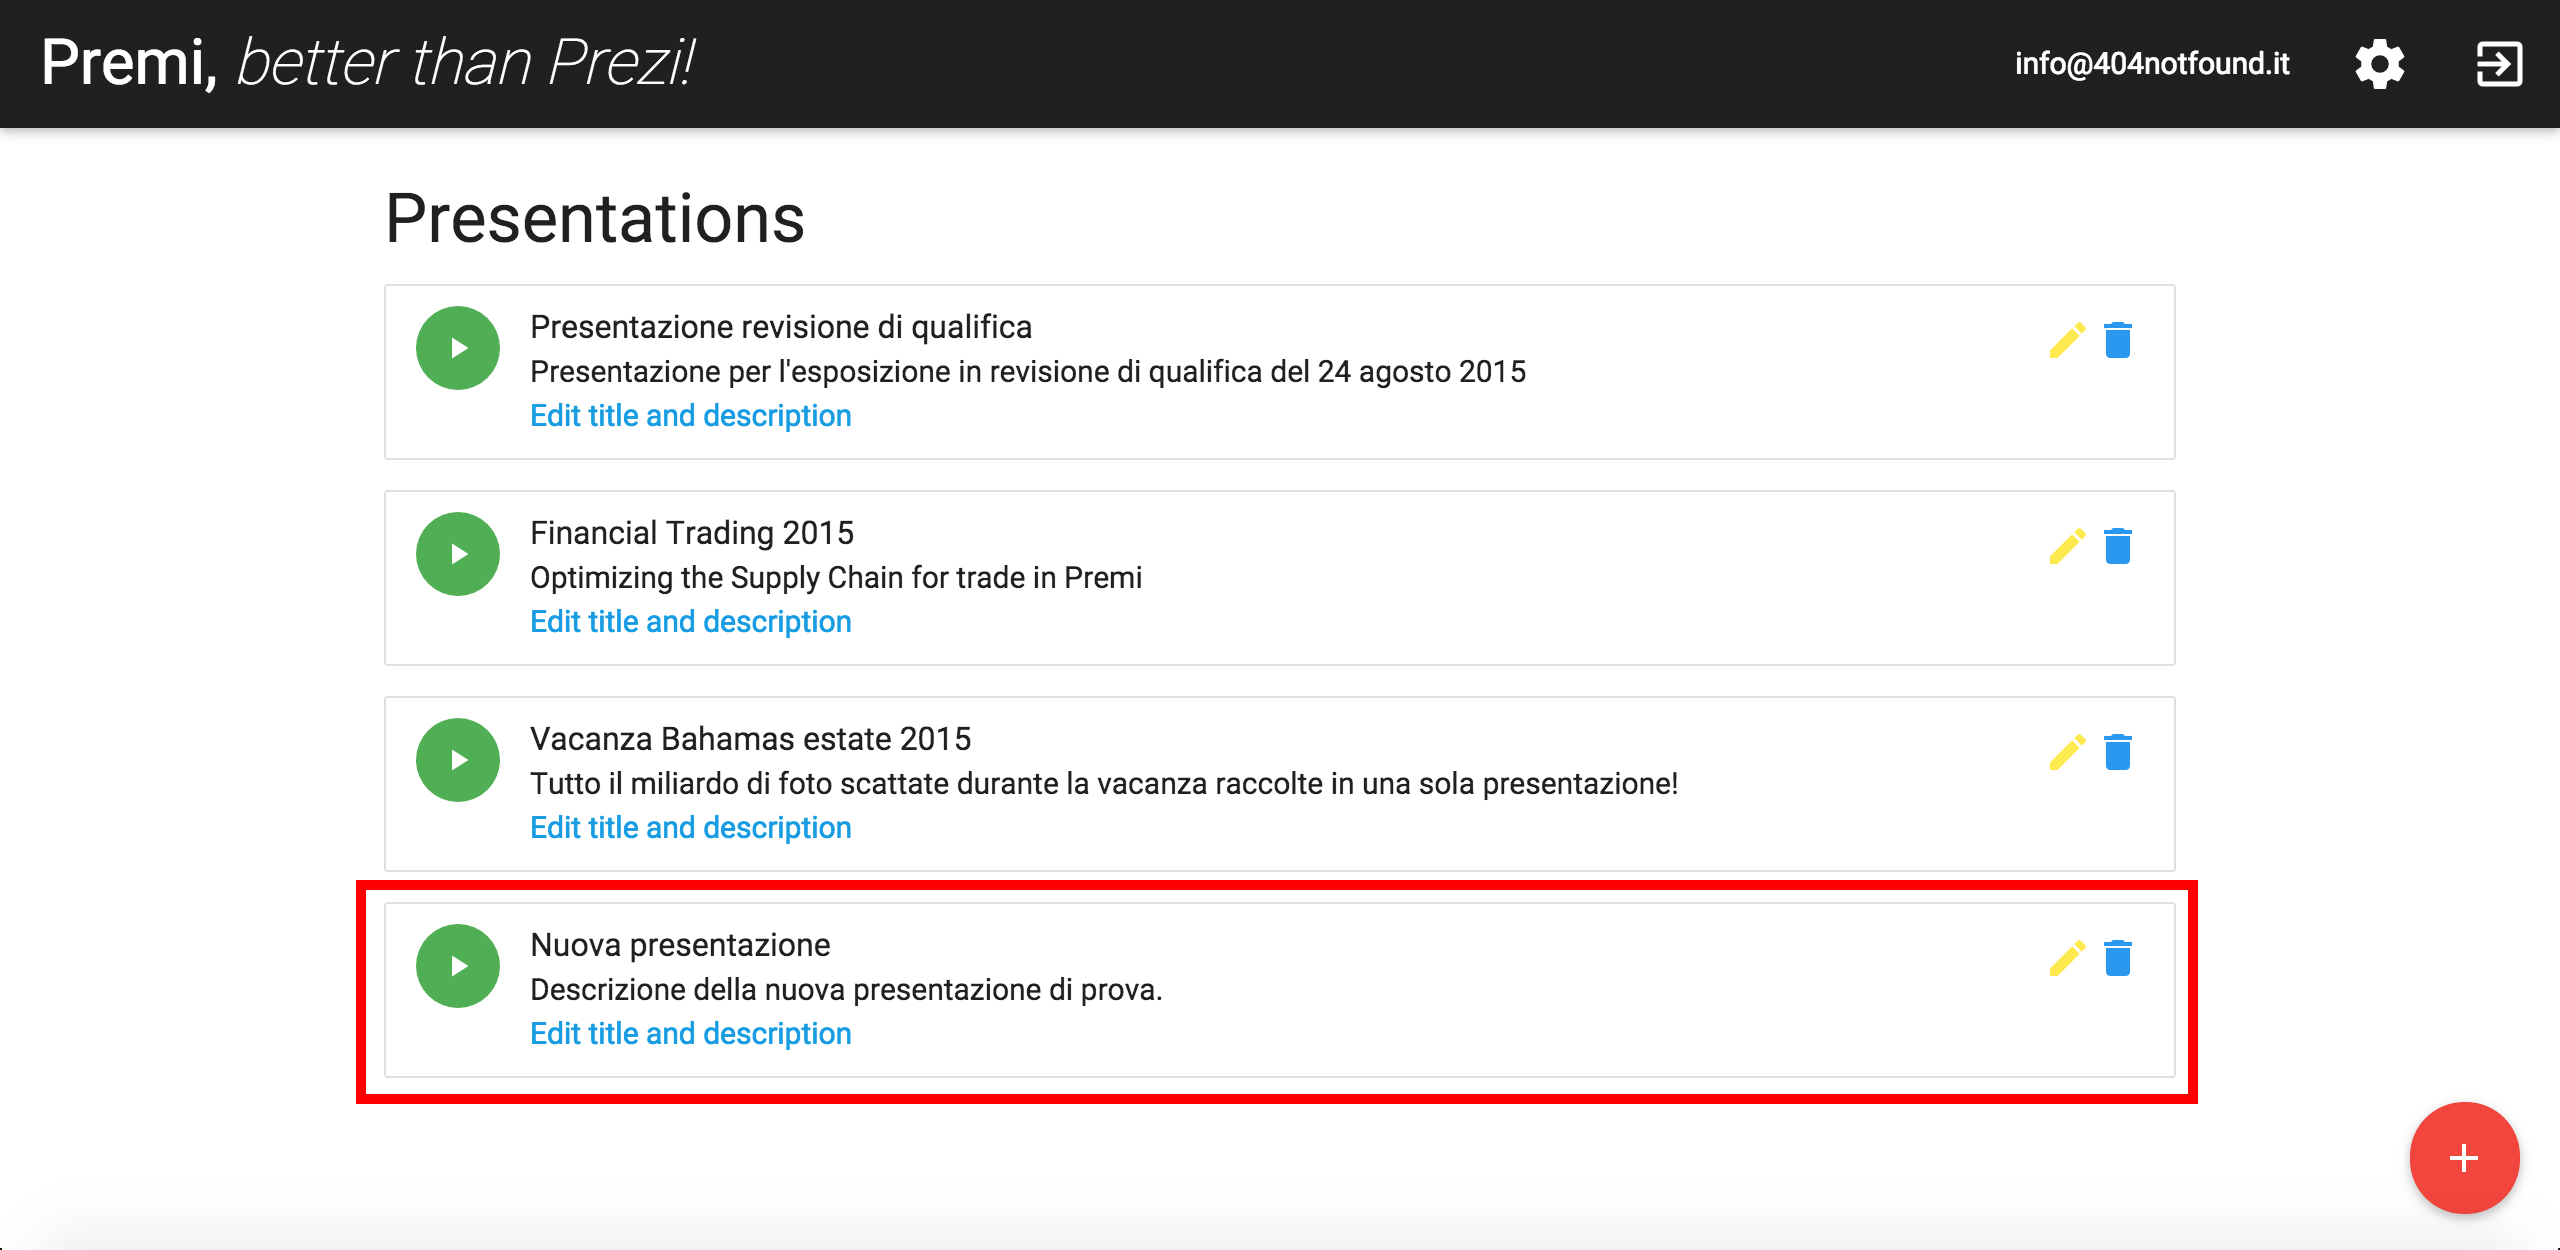
\includegraphics[scale=0.35]{img/list.png}
\caption{Lista presentazioni.}
\end{center}
\end{figure}

Ogni presentazione ha a disposizione tre azioni:\\

\begin{tabular}{ c l }
\parbox[c]{2em}{
\includegraphics[scale=0.4]{img/play.png}} & Avvia la presentazione;\\
\parbox[c]{2em}{
\includegraphics[scale=0.7]{img/edit.png}} & Modifica la presentazione. Apre la modalità editor;\\
\parbox[c]{2em}{
\includegraphics[scale=0.7]{img/delete.png}} & Elimina la presentazione. Segue richiesta di conferma.\\
\end{tabular}


\subsection{Editor}
L'editor di una presentazione sarà utilizzabile in tre modalità:

\begin{tabular}{ c p{15cm}}
\parbox[c]{2em}{
\includegraphics[scale=0.4]{img/frame_editor.png}} & \textbf{Frame editor}, che permette di aggiungere o modificare un frame selezionato, \newline aggiungendo a suo interno testo, immagini o forme;\\
\parbox[c]{2em}{
\includegraphics[scale=0.4]{img/info_editor.png}} & \textbf{Infographic editor}, che permette la modifica dell'infografica derivata dalla presentazione creata;\\
\parbox[c]{2em}{
\includegraphics[scale=0.4]{img/trails_editor.png}} & \textbf{Trails editor}, che permette di gestire i cammini presentativi presenti all'interno della presentazione.\\
\end{tabular}

\subsection{Frame editor}
\subsubsection{Aggiunta frame}
\subsubsection{Aggiunta elemento shape}
\subsubsection{Aggiunta testo}
\subsubsection{Modifica degli elementi}

\subsection{Infographic editor}

\subsection{Trails editor}

\subsubsection{Creazione percorso presentativo}


\subsection{Gestione presentazioni}
\subsubsection{Eliminazione}
\subsubsection{Modifica}

\subsection{Esportazione}
\subsubsection{Formato 1 (portable?)}
Spiegare anche come eventualmente visualizzare la presentazione in caso di formato portable.
\subsubsection{Formato 2 (poster?)}

\subsection{Avvio di una presentazione}
\subsubsection{Sessione locale}
\subsubsection{Sessione remota}

\subsection{Condivisione di una presentazione}

\subsection{Gestione dati account}

\subsection{Errori e loro cause}

